\documentclass[12pt]{article}\usepackage[]{graphicx}\usepackage[]{color}
% maxwidth is the original width if it is less than linewidth
% otherwise use linewidth (to make sure the graphics do not exceed the margin)
\makeatletter
\def\maxwidth{ %
  \ifdim\Gin@nat@width>\linewidth
    \linewidth
  \else
    \Gin@nat@width
  \fi
}
\makeatother

\definecolor{fgcolor}{rgb}{0.345, 0.345, 0.345}
\newcommand{\hlnum}[1]{\textcolor[rgb]{0.686,0.059,0.569}{#1}}%
\newcommand{\hlstr}[1]{\textcolor[rgb]{0.192,0.494,0.8}{#1}}%
\newcommand{\hlcom}[1]{\textcolor[rgb]{0.678,0.584,0.686}{\textit{#1}}}%
\newcommand{\hlopt}[1]{\textcolor[rgb]{0,0,0}{#1}}%
\newcommand{\hlstd}[1]{\textcolor[rgb]{0.345,0.345,0.345}{#1}}%
\newcommand{\hlkwa}[1]{\textcolor[rgb]{0.161,0.373,0.58}{\textbf{#1}}}%
\newcommand{\hlkwb}[1]{\textcolor[rgb]{0.69,0.353,0.396}{#1}}%
\newcommand{\hlkwc}[1]{\textcolor[rgb]{0.333,0.667,0.333}{#1}}%
\newcommand{\hlkwd}[1]{\textcolor[rgb]{0.737,0.353,0.396}{\textbf{#1}}}%
\let\hlipl\hlkwb

\usepackage{framed}
\makeatletter
\newenvironment{kframe}{%
 \def\at@end@of@kframe{}%
 \ifinner\ifhmode%
  \def\at@end@of@kframe{\end{minipage}}%
  \begin{minipage}{\columnwidth}%
 \fi\fi%
 \def\FrameCommand##1{\hskip\@totalleftmargin \hskip-\fboxsep
 \colorbox{shadecolor}{##1}\hskip-\fboxsep
     % There is no \\@totalrightmargin, so:
     \hskip-\linewidth \hskip-\@totalleftmargin \hskip\columnwidth}%
 \MakeFramed {\advance\hsize-\width
   \@totalleftmargin\z@ \linewidth\hsize
   \@setminipage}}%
 {\par\unskip\endMakeFramed%
 \at@end@of@kframe}
\makeatother

\definecolor{shadecolor}{rgb}{.97, .97, .97}
\definecolor{messagecolor}{rgb}{0, 0, 0}
\definecolor{warningcolor}{rgb}{1, 0, 1}
\definecolor{errorcolor}{rgb}{1, 0, 0}
\newenvironment{knitrout}{}{} % an empty environment to be redefined in TeX

\usepackage{alltt}
 
\usepackage[margin=1in]{geometry}
\usepackage{amsmath,amsthm,amssymb, mathtools}
\usepackage[T1]{fontenc}
\usepackage{lmodern}
\usepackage{fixltx2e}
\usepackage[shortlabels]{enumitem}
 
\newcommand{\N}{\mathbb{N}}
\newcommand{\R}{\mathbb{R}}
\newcommand{\Z}{\mathbb{Z}}
\newcommand{\Q}{\mathbb{Q}}

\newenvironment{theorem}[2][Theorem]{\begin{trivlist}
\item[\hskip \labelsep {\bfseries #1}\hskip \labelsep {\bfseries #2.}]}{\end{trivlist}}
\newenvironment{lemma}[2][Lemma]{\begin{trivlist}
\item[\hskip \labelsep {\bfseries #1}\hskip \labelsep {\bfseries #2.}]}{\end{trivlist}}
\newenvironment{exercise}[2][Exercise]{\begin{trivlist}
\item[\hskip \labelsep {\bfseries #1}\hskip \labelsep {\bfseries #2.}]}{\end{trivlist}}
\newenvironment{problem}[2][Problem]{\begin{trivlist}
\item[\hskip \labelsep {\bfseries #1}\hskip \labelsep {\bfseries #2.}]}{\end{trivlist}}
\newenvironment{question}[2][Question]{\begin{trivlist}
\item[\hskip \labelsep {\bfseries #1}\hskip \labelsep {\bfseries #2.}]}{\end{trivlist}}
\newenvironment{corollary}[2][Corollary]{\begin{trivlist}
\item[\hskip \labelsep {\bfseries #1}\hskip \labelsep {\bfseries #2.}]}{\end{trivlist}}
\newcommand{\textfrac}[2]{\dfrac{\text{#1}}{\text{#2}}}
\IfFileExists{upquote.sty}{\usepackage{upquote}}{}
\begin{document}

\title{Ch. 8 - Tree-Based Methods}

\author{Chris Hayduk}
\date{\today}

\maketitle



\section{Fitting Classification Trees}

We first use classification trees to analyze the \texttt{Carseats} data set. In these data, \texttt{Sales} is a continuous variable, and so we begin by recoding it as a binary variable. We use the \texttt{ifelse()} function to create a variable, called \texttt{High}, which takes on a value of Yes if the \texttt{Sales} variable exceeds 8, and takes on a value of No otherwise,

\begin{knitrout}
\definecolor{shadecolor}{rgb}{0.969, 0.969, 0.969}\color{fgcolor}\begin{kframe}
\begin{alltt}
\hlkwd{data}\hlstd{(Carseats)}
\hlkwd{attach}\hlstd{(Carseats)}
\hlstd{High} \hlkwb{=} \hlkwd{ifelse}\hlstd{(Sales}\hlopt{<=}\hlnum{8}\hlstd{,} \hlstr{"No"}\hlstd{,} \hlstr{"Yes"}\hlstd{)}
\end{alltt}
\end{kframe}
\end{knitrout}

Finally, we use the \texttt{data.frame()} function to merge \texttt{High} with the rest of the \texttt{Carseats} data.

\begin{knitrout}
\definecolor{shadecolor}{rgb}{0.969, 0.969, 0.969}\color{fgcolor}\begin{kframe}
\begin{alltt}
\hlstd{Carseats} \hlkwb{=} \hlkwd{data.frame}\hlstd{(Carseats,} \hlkwc{High}\hlstd{=}\hlkwd{as.factor}\hlstd{(High))}
\end{alltt}
\end{kframe}
\end{knitrout}

We now use the \texttt{tree()} function to fit a classification tree in order to predict \texttt{High} using all variables but \texttt{Sales}. The syntax of the \texttt{tree()} function is quite similar to that of the \texttt{lm()} function.

\begin{knitrout}
\definecolor{shadecolor}{rgb}{0.969, 0.969, 0.969}\color{fgcolor}\begin{kframe}
\begin{alltt}
\hlstd{tree.carseats} \hlkwb{=} \hlkwd{tree}\hlstd{(High}\hlopt{~}\hlstd{.}\hlopt{-}\hlstd{Sales,} \hlkwc{data}\hlstd{=Carseats)}
\end{alltt}
\end{kframe}
\end{knitrout}

The \texttt{Summary()} function lists the variables that are used as internal nodes in the tree, the number of terminal nodes, and the training error rate.
\begin{knitrout}
\definecolor{shadecolor}{rgb}{0.969, 0.969, 0.969}\color{fgcolor}\begin{kframe}
\begin{alltt}
\hlkwd{summary}\hlstd{(tree.carseats)}
\end{alltt}
\begin{verbatim}
## 
## Classification tree:
## tree(formula = High ~ . - Sales, data = Carseats)
## Variables actually used in tree construction:
## [1] "ShelveLoc"   "Price"       "Income"      "CompPrice"   "Population" 
## [6] "Advertising" "Age"         "US"         
## Number of terminal nodes:  27 
## Residual mean deviance:  0.4575 = 170.7 / 373 
## Misclassification error rate: 0.09 = 36 / 400
\end{verbatim}
\end{kframe}
\end{knitrout}

We see that the training error rate is 9\%. For classification trees, the deviance reported in the output of \texttt{summary()} is given by,
\begin{align}
-2 \sum_m \sum_k n_{mk} \log \hat{p}_{mk}
\end{align}

where $n_{mk}$ is the number of observations in the $m$th terminal node that belong to the $k$th class. A small deviance indicates a tree that provides a good fit to the (training) data. The \textit{residual mean deviance} reported is simply the deviance divided by $n - |T_0|$, which in this case is $400-27=373$.


One of the most attractive properties of trees is that they can be graphically displayed. We use the \texttt{plot()} function to display the tree structure, and the \texttt{text()} function to display the node labels. The argument \texttt{pretty=0} instructs \texttt{R} to include the category names for any qualitative predictors, rather than simply displaying a letter for each category.

\begin{knitrout}
\definecolor{shadecolor}{rgb}{0.969, 0.969, 0.969}\color{fgcolor}\begin{kframe}
\begin{alltt}
\hlkwd{plot}\hlstd{(tree.carseats)}
\hlkwd{text}\hlstd{(tree.carseats,} \hlkwc{pretty} \hlstd{=} \hlnum{0}\hlstd{)}
\end{alltt}
\end{kframe}
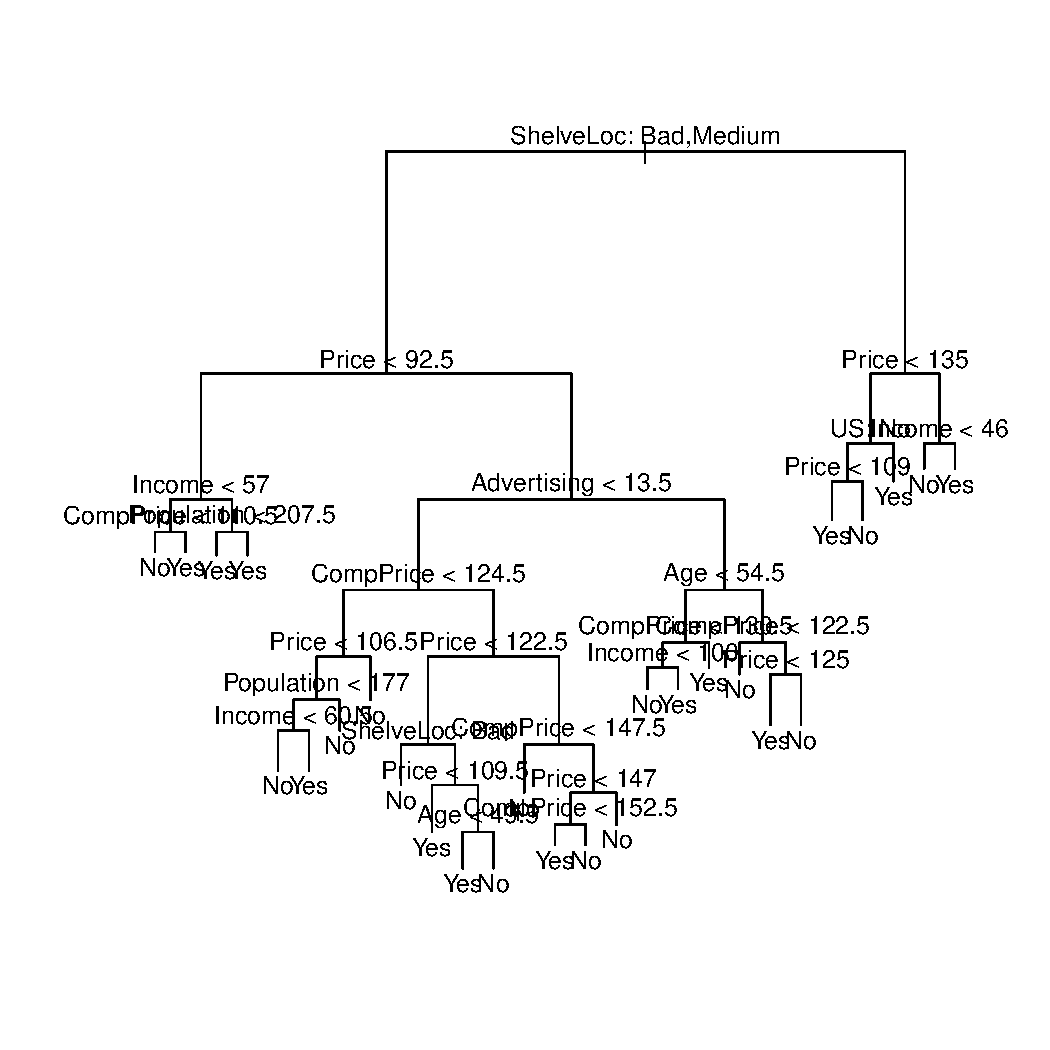
\includegraphics[width=\maxwidth]{figure/unnamed-chunk-6-1} 

\end{knitrout}

The most important indicator of \texttt{Sales} appears to be shelving location, since the first branch differentiates Good locations from Bad and Medium locations.

If we just type the name of the tree object, \texttt{R} prints output corresponding to each branch of the tree. \texttt{R} displays the split criterion (e.g. \texttt{Price<92.5}), the number of observations in that branch, the deviance the overall preduction for that branch (Yes or No), and the fraction of observations in that branch that take on values of Yes and No. Branches that lead to terminal nodes are indicated using asteriks.

\begin{knitrout}
\definecolor{shadecolor}{rgb}{0.969, 0.969, 0.969}\color{fgcolor}\begin{kframe}
\begin{alltt}
\hlstd{tree.carseats}
\end{alltt}
\begin{verbatim}
## node), split, n, deviance, yval, (yprob)
##       * denotes terminal node
## 
##   1) root 400 541.500 No ( 0.59000 0.41000 )  
##     2) ShelveLoc: Bad,Medium 315 390.600 No ( 0.68889 0.31111 )  
##       4) Price < 92.5 46  56.530 Yes ( 0.30435 0.69565 )  
##         8) Income < 57 10  12.220 No ( 0.70000 0.30000 )  
##          16) CompPrice < 110.5 5   0.000 No ( 1.00000 0.00000 ) *
##          17) CompPrice > 110.5 5   6.730 Yes ( 0.40000 0.60000 ) *
##         9) Income > 57 36  35.470 Yes ( 0.19444 0.80556 )  
##          18) Population < 207.5 16  21.170 Yes ( 0.37500 0.62500 ) *
##          19) Population > 207.5 20   7.941 Yes ( 0.05000 0.95000 ) *
##       5) Price > 92.5 269 299.800 No ( 0.75465 0.24535 )  
##        10) Advertising < 13.5 224 213.200 No ( 0.81696 0.18304 )  
##          20) CompPrice < 124.5 96  44.890 No ( 0.93750 0.06250 )  
##            40) Price < 106.5 38  33.150 No ( 0.84211 0.15789 )  
##              80) Population < 177 12  16.300 No ( 0.58333 0.41667 )  
##               160) Income < 60.5 6   0.000 No ( 1.00000 0.00000 ) *
##               161) Income > 60.5 6   5.407 Yes ( 0.16667 0.83333 ) *
##              81) Population > 177 26   8.477 No ( 0.96154 0.03846 ) *
##            41) Price > 106.5 58   0.000 No ( 1.00000 0.00000 ) *
##          21) CompPrice > 124.5 128 150.200 No ( 0.72656 0.27344 )  
##            42) Price < 122.5 51  70.680 Yes ( 0.49020 0.50980 )  
##              84) ShelveLoc: Bad 11   6.702 No ( 0.90909 0.09091 ) *
##              85) ShelveLoc: Medium 40  52.930 Yes ( 0.37500 0.62500 )  
##               170) Price < 109.5 16   7.481 Yes ( 0.06250 0.93750 ) *
##               171) Price > 109.5 24  32.600 No ( 0.58333 0.41667 )  
##                 342) Age < 49.5 13  16.050 Yes ( 0.30769 0.69231 ) *
##                 343) Age > 49.5 11   6.702 No ( 0.90909 0.09091 ) *
##            43) Price > 122.5 77  55.540 No ( 0.88312 0.11688 )  
##              86) CompPrice < 147.5 58  17.400 No ( 0.96552 0.03448 ) *
##              87) CompPrice > 147.5 19  25.010 No ( 0.63158 0.36842 )  
##               174) Price < 147 12  16.300 Yes ( 0.41667 0.58333 )  
##                 348) CompPrice < 152.5 7   5.742 Yes ( 0.14286 0.85714 ) *
##                 349) CompPrice > 152.5 5   5.004 No ( 0.80000 0.20000 ) *
##               175) Price > 147 7   0.000 No ( 1.00000 0.00000 ) *
##        11) Advertising > 13.5 45  61.830 Yes ( 0.44444 0.55556 )  
##          22) Age < 54.5 25  25.020 Yes ( 0.20000 0.80000 )  
##            44) CompPrice < 130.5 14  18.250 Yes ( 0.35714 0.64286 )  
##              88) Income < 100 9  12.370 No ( 0.55556 0.44444 ) *
##              89) Income > 100 5   0.000 Yes ( 0.00000 1.00000 ) *
##            45) CompPrice > 130.5 11   0.000 Yes ( 0.00000 1.00000 ) *
##          23) Age > 54.5 20  22.490 No ( 0.75000 0.25000 )  
##            46) CompPrice < 122.5 10   0.000 No ( 1.00000 0.00000 ) *
##            47) CompPrice > 122.5 10  13.860 No ( 0.50000 0.50000 )  
##              94) Price < 125 5   0.000 Yes ( 0.00000 1.00000 ) *
##              95) Price > 125 5   0.000 No ( 1.00000 0.00000 ) *
##     3) ShelveLoc: Good 85  90.330 Yes ( 0.22353 0.77647 )  
##       6) Price < 135 68  49.260 Yes ( 0.11765 0.88235 )  
##        12) US: No 17  22.070 Yes ( 0.35294 0.64706 )  
##          24) Price < 109 8   0.000 Yes ( 0.00000 1.00000 ) *
##          25) Price > 109 9  11.460 No ( 0.66667 0.33333 ) *
##        13) US: Yes 51  16.880 Yes ( 0.03922 0.96078 ) *
##       7) Price > 135 17  22.070 No ( 0.64706 0.35294 )  
##        14) Income < 46 6   0.000 No ( 1.00000 0.00000 ) *
##        15) Income > 46 11  15.160 Yes ( 0.45455 0.54545 ) *
\end{verbatim}
\end{kframe}
\end{knitrout}

In order to properly evaluate the performance of a classification tree on these data, we must estimate the test error rather than simply computing the training error. We split the observations into a training set and a test set, build the tree using the training set, and evaluate its performance on the test data.
\begin{knitrout}
\definecolor{shadecolor}{rgb}{0.969, 0.969, 0.969}\color{fgcolor}\begin{kframe}
\begin{alltt}
\hlkwd{set.seed}\hlstd{(}\hlnum{2}\hlstd{)}
\hlstd{train} \hlkwb{=} \hlkwd{sample}\hlstd{(}\hlnum{1}\hlopt{:}\hlkwd{nrow}\hlstd{(Carseats),} \hlnum{200}\hlstd{)}
\hlstd{Carseats.test} \hlkwb{=} \hlstd{Carseats[}\hlopt{-}\hlstd{train,]}
\hlstd{High.test} \hlkwb{=} \hlstd{High[}\hlopt{-}\hlstd{train]}
\hlstd{tree.carseats}\hlkwb{=}\hlkwd{tree}\hlstd{(High}\hlopt{~}\hlstd{.}\hlopt{-}\hlstd{Sales, Carseats,} \hlkwc{subset} \hlstd{= train)}
\hlstd{tree.pred} \hlkwb{=} \hlkwd{predict}\hlstd{(tree.carseats, Carseats.test,} \hlkwc{type}\hlstd{=}\hlstr{"class"}\hlstd{)}
\hlkwd{table}\hlstd{(tree.pred, High.test)}
\end{alltt}
\begin{verbatim}
##          High.test
## tree.pred  No Yes
##       No  104  33
##       Yes  13  50
\end{verbatim}
\end{kframe}
\end{knitrout}

Next, we consider whether pruning the tree might lead to improved results. The function \texttt{cv.tree()} performs cross validation in order to determine the optimal level of tree complexity.

\begin{knitrout}
\definecolor{shadecolor}{rgb}{0.969, 0.969, 0.969}\color{fgcolor}\begin{kframe}
\begin{alltt}
\hlkwd{set.seed}\hlstd{(}\hlnum{3}\hlstd{)}
\hlstd{cv.carseats}\hlkwb{=}\hlkwd{cv.tree}\hlstd{(tree.carseats,}\hlkwc{FUN}\hlstd{=prune.misclass)}
\hlkwd{names}\hlstd{(cv.carseats)}
\end{alltt}
\begin{verbatim}
## [1] "size"   "dev"    "k"      "method"
\end{verbatim}
\end{kframe}
\end{knitrout}

Note that, despite the name, \texttt{dev} corresponds to the cross-validation error rate in this instance. The tree with 9 terminal nodes results in the lowest cross-validation error rate, with 50 cross-validation errors. We plot the error rate as a function of both \texttt{size} and \texttt{k}.

\begin{knitrout}
\definecolor{shadecolor}{rgb}{0.969, 0.969, 0.969}\color{fgcolor}\begin{kframe}
\begin{alltt}
\hlkwd{par}\hlstd{(}\hlkwc{mfrow}\hlstd{=}\hlkwd{c}\hlstd{(}\hlnum{1}\hlstd{,}\hlnum{2}\hlstd{))}
\hlkwd{plot}\hlstd{(cv.carseats}\hlopt{$}\hlstd{size,cv.carseats}\hlopt{$}\hlstd{dev,}\hlkwc{type}\hlstd{=}\hlstr{"b"}\hlstd{)}
\hlkwd{plot}\hlstd{(cv.carseats}\hlopt{$}\hlstd{k, cv.carseats}\hlopt{$}\hlstd{dev,} \hlkwc{type}\hlstd{=}\hlstr{"b"}\hlstd{)}
\end{alltt}
\end{kframe}
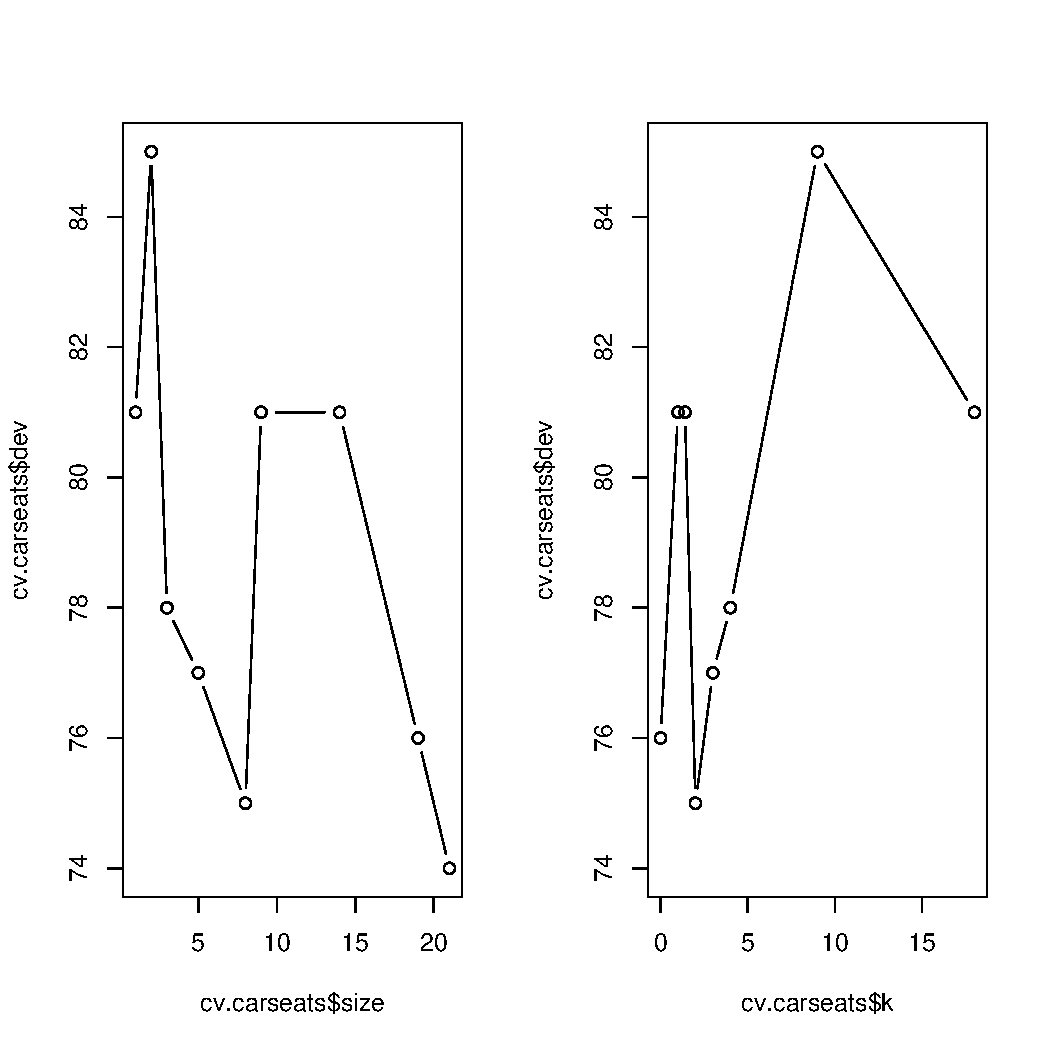
\includegraphics[width=\maxwidth]{figure/unnamed-chunk-10-1} 

\end{knitrout}

We now apply the \texttt{prune.misclass()} function in order to prune the tree to obtain the nine-node tree.

\begin{knitrout}
\definecolor{shadecolor}{rgb}{0.969, 0.969, 0.969}\color{fgcolor}\begin{kframe}
\begin{alltt}
\hlstd{prune.carseats}\hlkwb{=}\hlkwd{prune.misclass}\hlstd{(tree.carseats,}\hlkwc{best}\hlstd{=}\hlnum{9}\hlstd{)}
\hlkwd{plot}\hlstd{(prune.carseats)}
\hlkwd{text}\hlstd{(prune.carseats,} \hlkwc{pretty}\hlstd{=}\hlnum{0}\hlstd{)}
\end{alltt}
\end{kframe}
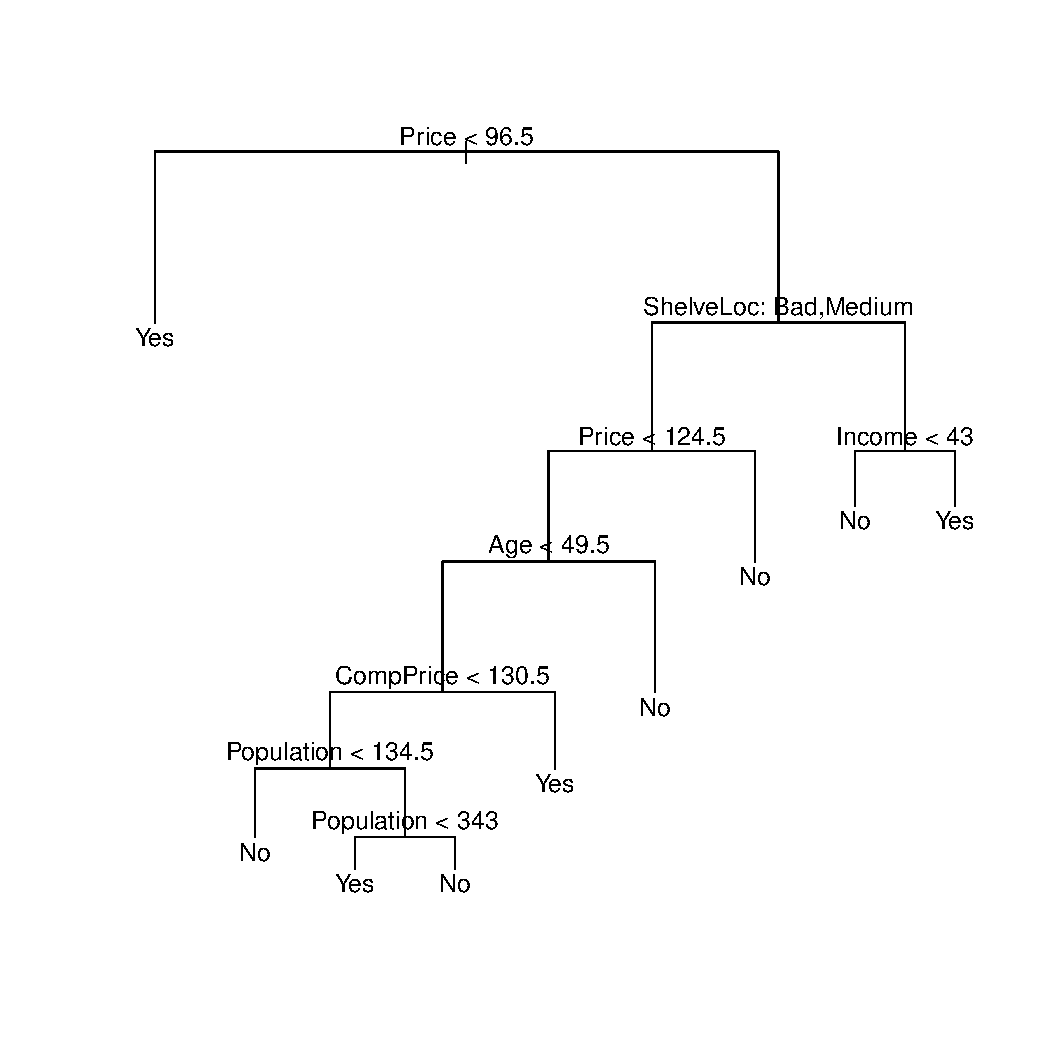
\includegraphics[width=\maxwidth]{figure/unnamed-chunk-11-1} 

\end{knitrout}

How well does this pruned tree perform on the test data set? Once again, we apply the \texttt{predict()} function.

\begin{knitrout}
\definecolor{shadecolor}{rgb}{0.969, 0.969, 0.969}\color{fgcolor}\begin{kframe}
\begin{alltt}
\hlstd{tree.pred}\hlkwb{=}\hlkwd{predict}\hlstd{(prune.carseats, Carseats.test,} \hlkwc{type}\hlstd{=}\hlstr{"class"}\hlstd{)}
\hlkwd{table}\hlstd{(tree.pred, High.test)}
\end{alltt}
\begin{verbatim}
##          High.test
## tree.pred No Yes
##       No  97  25
##       Yes 20  58
\end{verbatim}
\end{kframe}
\end{knitrout}

Now 77\% of the test observations are correctly classified, so not only has the pruning process produced a more interpretable tree, but it has also improved the classification accuracy.

If we increase the value of \texttt{best}, we obtain a larger pruned tree with lower classification accuracy:
\begin{knitrout}
\definecolor{shadecolor}{rgb}{0.969, 0.969, 0.969}\color{fgcolor}\begin{kframe}
\begin{alltt}
\hlstd{prune.carseats} \hlkwb{=} \hlkwd{prune.misclass}\hlstd{(tree.carseats,} \hlkwc{best} \hlstd{=} \hlnum{15}\hlstd{)}
\hlkwd{plot}\hlstd{(prune.carseats)}
\hlkwd{text}\hlstd{(prune.carseats,} \hlkwc{pretty}\hlstd{=}\hlnum{0}\hlstd{)}
\end{alltt}
\end{kframe}
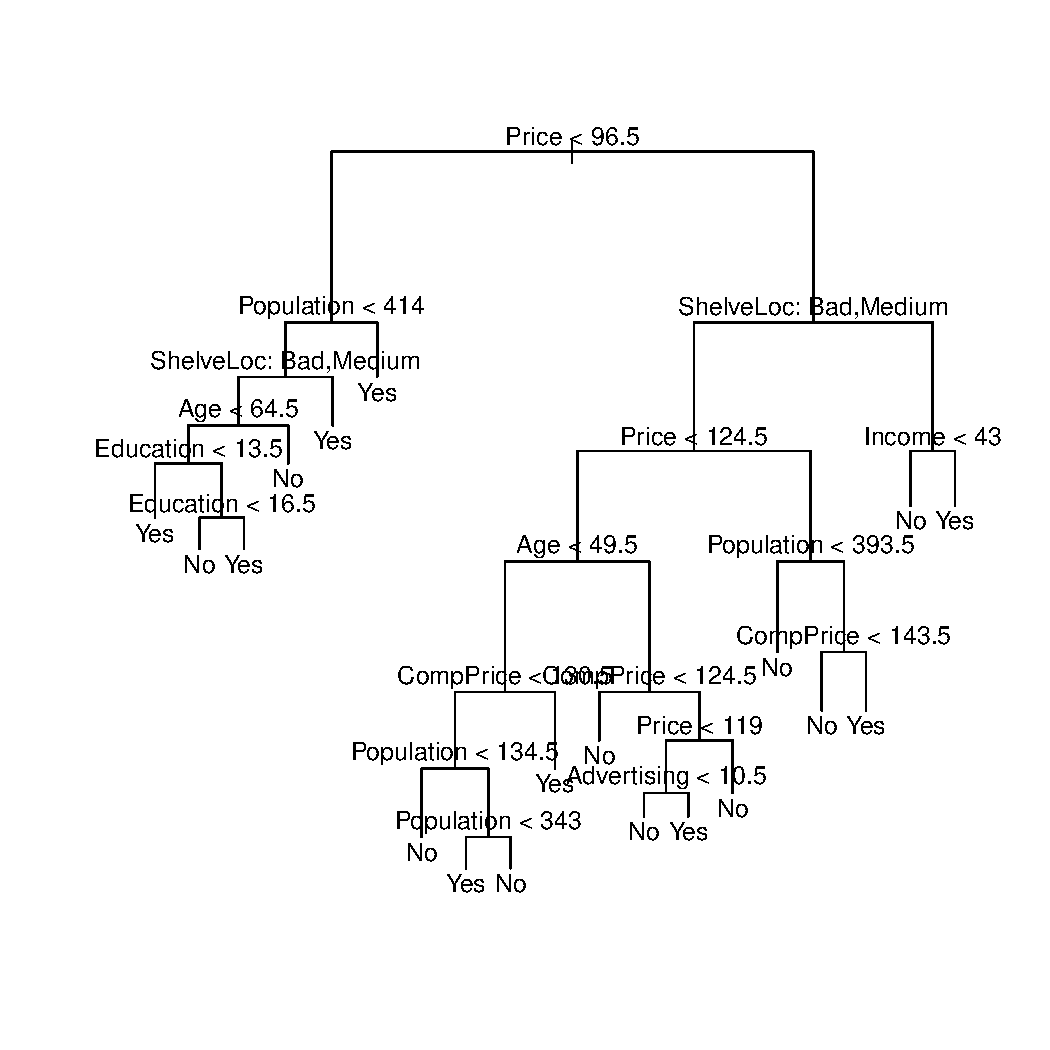
\includegraphics[width=\maxwidth]{figure/unnamed-chunk-13-1} 
\begin{kframe}\begin{alltt}
\hlstd{tree.pred}\hlkwb{=}\hlkwd{predict}\hlstd{(prune.carseats, Carseats.test,} \hlkwc{type}\hlstd{=}\hlstr{"class"}\hlstd{)}
\hlkwd{table}\hlstd{(tree.pred, High.test)}
\end{alltt}
\begin{verbatim}
##          High.test
## tree.pred  No Yes
##       No  102  30
##       Yes  15  53
\end{verbatim}
\end{kframe}
\end{knitrout}


\newpage
\section{Fitting Regression Trees}

Here we fit a regression tree to the \texttt{Boston} data set. First, we create a training set, and fit the tree to the training set.

\begin{knitrout}
\definecolor{shadecolor}{rgb}{0.969, 0.969, 0.969}\color{fgcolor}\begin{kframe}
\begin{alltt}
\hlkwd{set.seed}\hlstd{(}\hlnum{1}\hlstd{)}
\hlstd{train} \hlkwb{=} \hlkwd{sample}\hlstd{(}\hlnum{1}\hlopt{:}\hlkwd{nrow}\hlstd{(Boston),} \hlkwd{nrow}\hlstd{(Boston)}\hlopt{/}\hlnum{2}\hlstd{)}
\hlstd{tree.boston} \hlkwb{=} \hlkwd{tree}\hlstd{(medv}\hlopt{~}\hlstd{., Boston,} \hlkwc{subset}\hlstd{=train)}
\hlkwd{summary}\hlstd{(tree.boston)}
\end{alltt}
\begin{verbatim}
## 
## Regression tree:
## tree(formula = medv ~ ., data = Boston, subset = train)
## Variables actually used in tree construction:
## [1] "rm"    "lstat" "crim"  "age"  
## Number of terminal nodes:  7 
## Residual mean deviance:  10.38 = 2555 / 246 
## Distribution of residuals:
##     Min.  1st Qu.   Median     Mean  3rd Qu.     Max. 
## -10.1800  -1.7770  -0.1775   0.0000   1.9230  16.5800
\end{verbatim}
\end{kframe}
\end{knitrout}

Note that the output of \texttt{summary()} indicates that only three of the variables have been used in constructing the tree. In the context of a regression tree, the deviance is simply the sum of squared errors for the tree. We now plot the tree.

\begin{knitrout}
\definecolor{shadecolor}{rgb}{0.969, 0.969, 0.969}\color{fgcolor}\begin{kframe}
\begin{alltt}
\hlkwd{plot}\hlstd{(tree.boston)}
\hlkwd{text}\hlstd{(tree.boston,} \hlkwc{pretty}\hlstd{=}\hlnum{0}\hlstd{)}
\end{alltt}
\end{kframe}
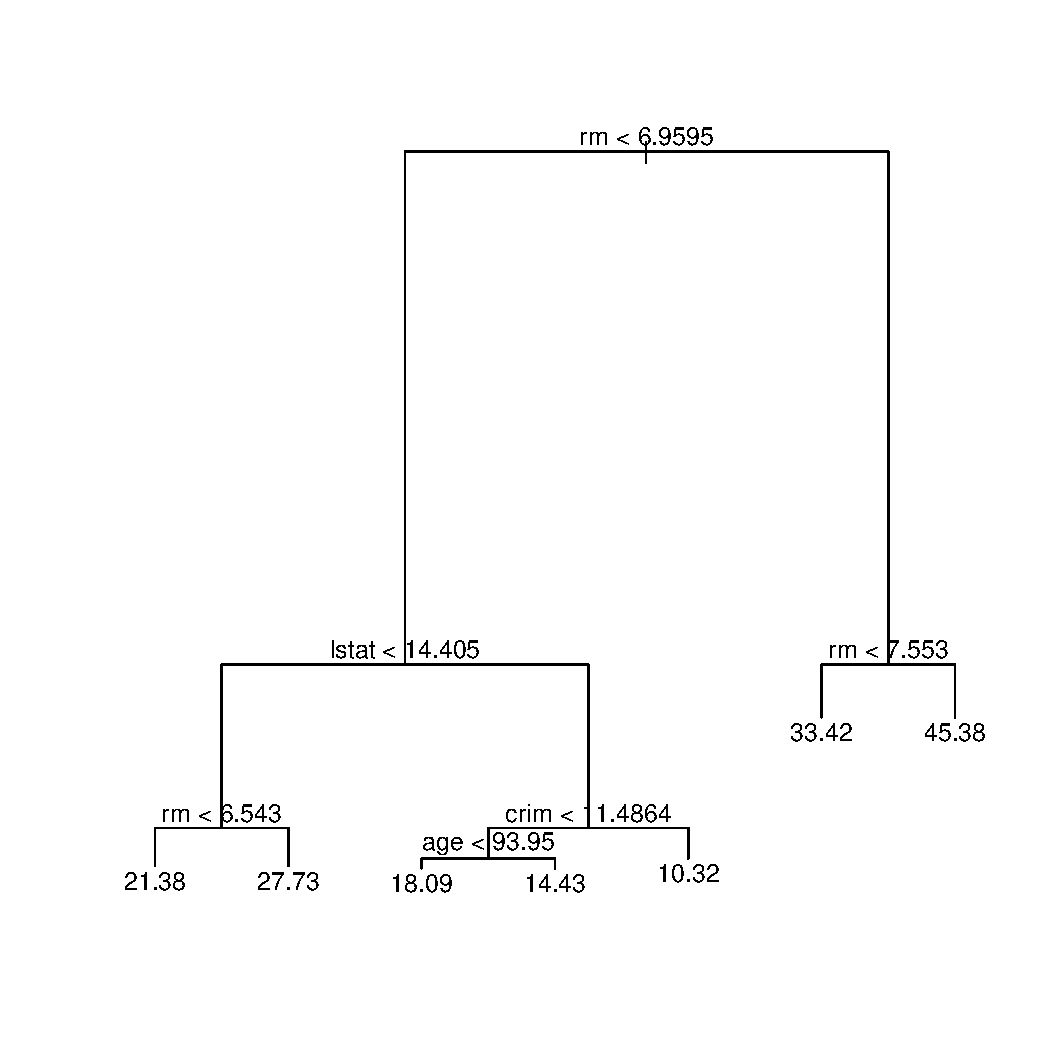
\includegraphics[width=\maxwidth]{figure/unnamed-chunk-15-1} 

\end{knitrout}

The variable \texttt{lstat} measures the percentage of individuals with lower socioeconomic status. The tree indicates that lower values of \texttt{lstat} correspond to more expensive houses. The tree predicts a median house price of \$46,400 for larger homes in suburbs in which residents have high socioeconomic status.

Now we use the \texttt{cv.tree()} function to see whether pruning the tree will improve performance.

\begin{knitrout}
\definecolor{shadecolor}{rgb}{0.969, 0.969, 0.969}\color{fgcolor}\begin{kframe}
\begin{alltt}
\hlstd{cv.boston} \hlkwb{=} \hlkwd{cv.tree}\hlstd{(tree.boston)}
\hlkwd{plot}\hlstd{(cv.boston}\hlopt{$}\hlstd{size, cv.boston}\hlopt{$}\hlstd{dev,} \hlkwc{type}\hlstd{=}\hlstr{'b'}\hlstd{)}
\end{alltt}
\end{kframe}
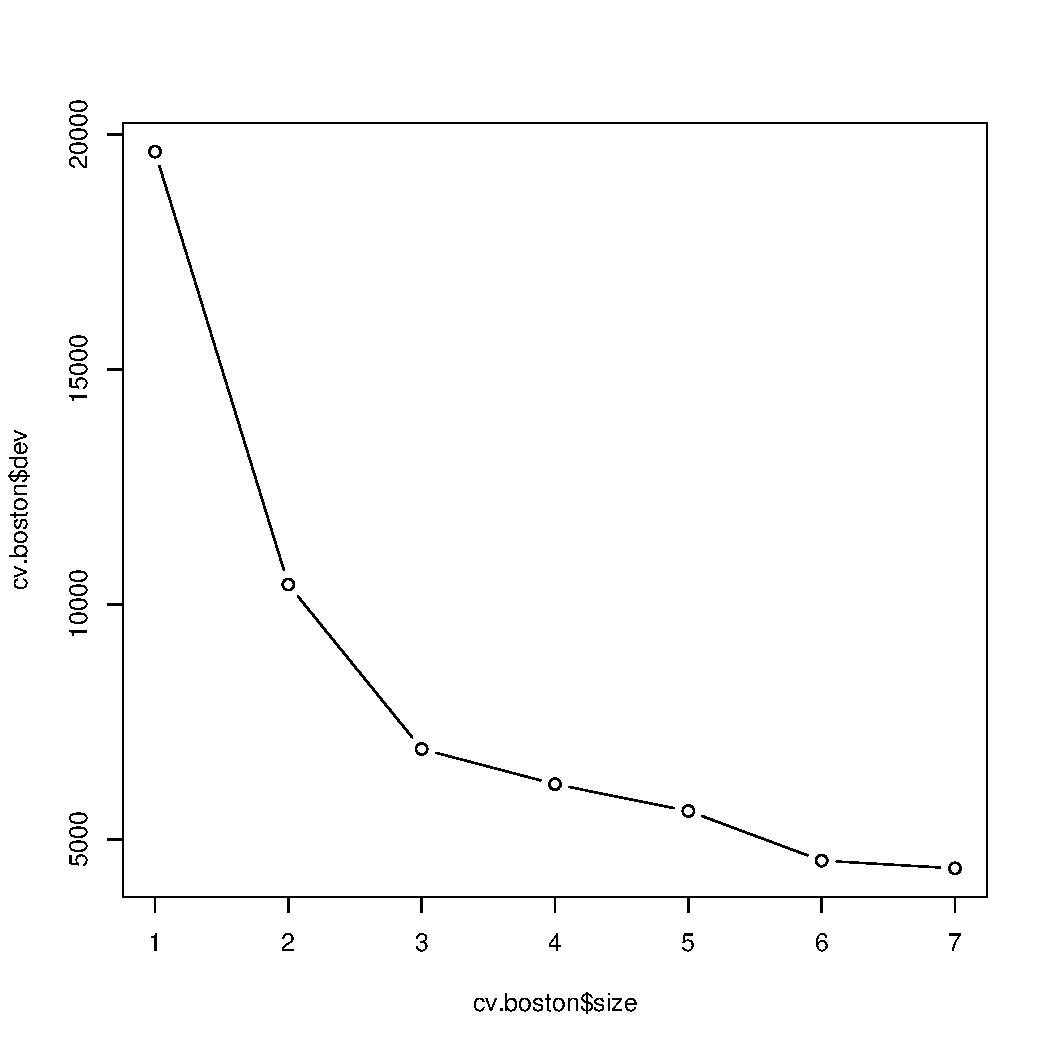
\includegraphics[width=\maxwidth]{figure/unnamed-chunk-16-1} 

\end{knitrout}

In this case, the most complex tree is selected by cross-validation. We can also prune the tree as follows:

\begin{knitrout}
\definecolor{shadecolor}{rgb}{0.969, 0.969, 0.969}\color{fgcolor}\begin{kframe}
\begin{alltt}
\hlstd{yhat} \hlkwb{=} \hlkwd{predict}\hlstd{(tree.boston,} \hlkwc{newdata}\hlstd{=Boston[}\hlopt{-}\hlstd{train,])}
\hlstd{boston.test} \hlkwb{=} \hlstd{Boston[}\hlopt{-}\hlstd{train,} \hlstr{"medv"}\hlstd{]}
\hlkwd{plot}\hlstd{(yhat, boston.test)}
\hlkwd{abline}\hlstd{(}\hlnum{0}\hlstd{,}\hlnum{1}\hlstd{)}
\end{alltt}
\end{kframe}
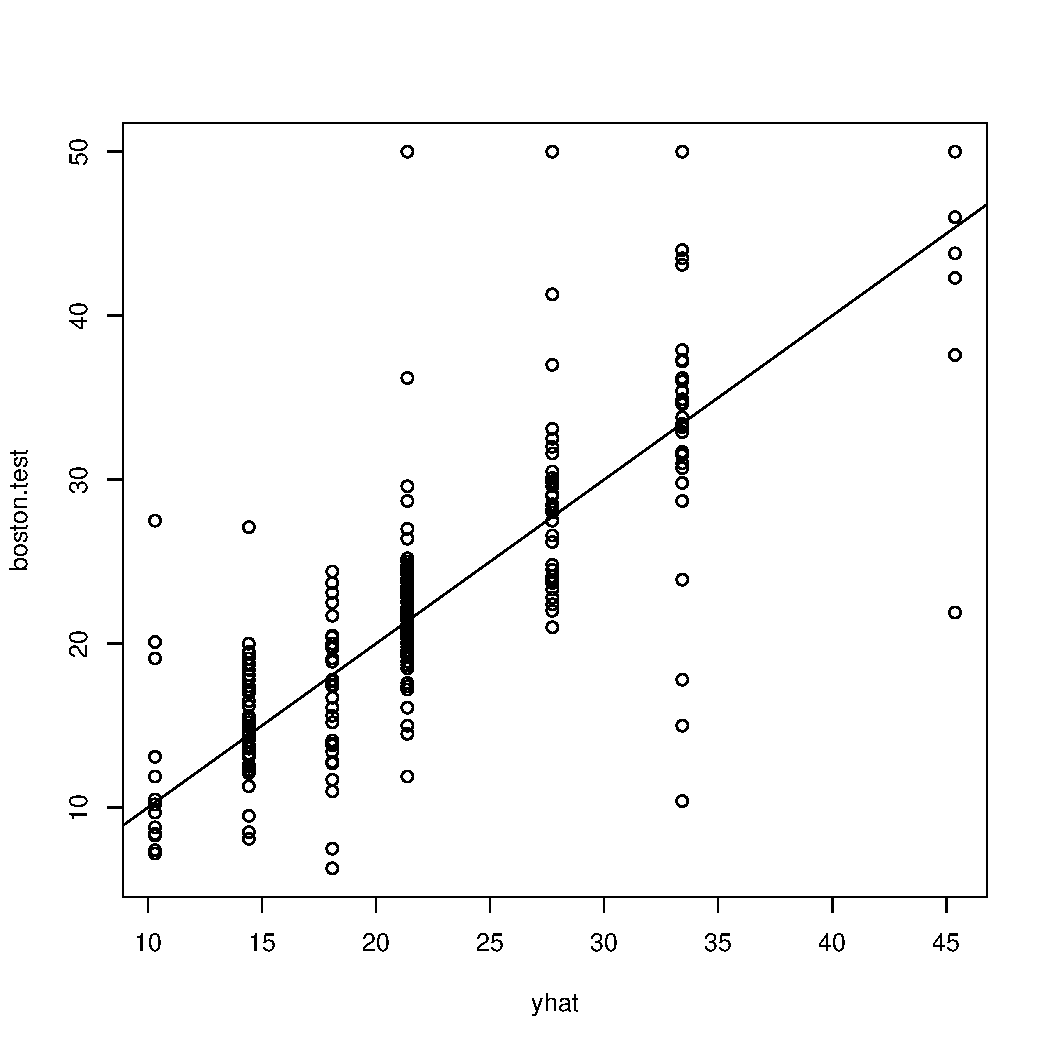
\includegraphics[width=\maxwidth]{figure/unnamed-chunk-17-1} 
\begin{kframe}\begin{alltt}
\hlkwd{mean}\hlstd{((yhat}\hlopt{-}\hlstd{boston.test)}\hlopt{^}\hlnum{2}\hlstd{)}
\end{alltt}
\begin{verbatim}
## [1] 35.28688
\end{verbatim}
\end{kframe}
\end{knitrout}

In other words, the test set MSE associated with the regression tree is 25.05. The square root of the MSE is therefore around 5.005, indicating that this model leads to test predictions that are within around \$5,005 of the true median home value for the suburb.

\newpage
\section{Bagging and Random Forests}

Here we apply bagging and random forests to the \texttt{Boston} data, using the \texttt{randomForest} package in \texttt{R}. The exact results obtained in this section may depend on the version of \texttt{R} and the version of the \texttt{randomForest} package. Recall that bagging is simply a special case of random forest with $m = p$. Therefore, the \texttt{randomForest()} function can be used to perform both random forests and bagging. We perform bagging as follows:

\begin{knitrout}
\definecolor{shadecolor}{rgb}{0.969, 0.969, 0.969}\color{fgcolor}\begin{kframe}
\begin{alltt}
\hlkwd{set.seed}\hlstd{(}\hlnum{1}\hlstd{)}
\hlstd{bag.boston} \hlkwb{=} \hlkwd{randomForest}\hlstd{(medv}\hlopt{~}\hlstd{.,}
                          \hlkwc{data}\hlstd{=Boston,}
                          \hlkwc{subset}\hlstd{=train,}
                          \hlkwc{mtry}\hlstd{=}\hlnum{13}\hlstd{,}
                          \hlkwc{importance}\hlstd{=}\hlnum{TRUE}\hlstd{)}
\hlstd{bag.boston}
\end{alltt}
\begin{verbatim}
## 
## Call:
##  randomForest(formula = medv ~ ., data = Boston, mtry = 13, importance = TRUE,      subset = train) 
##                Type of random forest: regression
##                      Number of trees: 500
## No. of variables tried at each split: 13
## 
##           Mean of squared residuals: 11.39601
##                     % Var explained: 85.17
\end{verbatim}
\end{kframe}
\end{knitrout}

The argument \texttt{mtry=13} indicates that all $13$ predictors should be considered for each split of the tree - in other words, that bagging should be done. How well does this bagged model perform on the test set?

\begin{knitrout}
\definecolor{shadecolor}{rgb}{0.969, 0.969, 0.969}\color{fgcolor}\begin{kframe}
\begin{alltt}
\hlstd{yhat.bag} \hlkwb{=} \hlkwd{predict}\hlstd{(bag.boston,} \hlkwc{newdata}\hlstd{=Boston[}\hlopt{-}\hlstd{train,])}
\hlkwd{plot}\hlstd{(yhat.bag, boston.test)}
\hlkwd{abline}\hlstd{(}\hlnum{0}\hlstd{,}\hlnum{1}\hlstd{)}
\end{alltt}
\end{kframe}
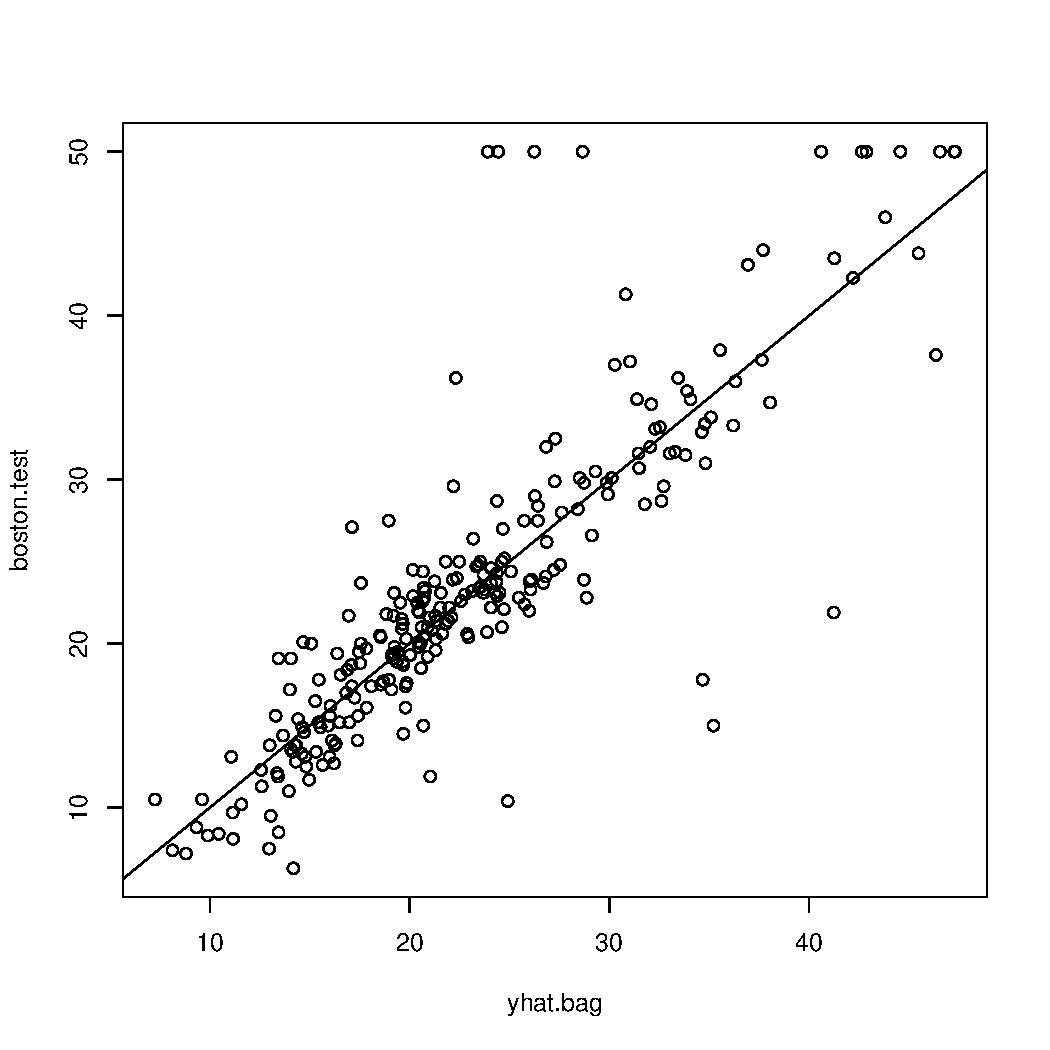
\includegraphics[width=\maxwidth]{figure/unnamed-chunk-19-1} 
\begin{kframe}\begin{alltt}
\hlkwd{mean}\hlstd{((yhat.bag}\hlopt{-}\hlstd{boston.test)}\hlopt{^}\hlnum{2}\hlstd{)}
\end{alltt}
\begin{verbatim}
## [1] 23.59273
\end{verbatim}
\end{kframe}
\end{knitrout}

The test MSE associated with the bagged regression tree is 13.16, almost half that obtained using an optimally-pruned single tree. We could change the number of trees grown by \texttt{randomForest()} using the \texttt{ntree} argument:

\begin{knitrout}
\definecolor{shadecolor}{rgb}{0.969, 0.969, 0.969}\color{fgcolor}\begin{kframe}
\begin{alltt}
\hlstd{bag.boston} \hlkwb{=} \hlkwd{randomForest}\hlstd{(medv}\hlopt{~}\hlstd{.,} \hlkwc{data}\hlstd{=Boston,}
                          \hlkwc{subset}\hlstd{=train,} \hlkwc{mtry}\hlstd{=}\hlnum{13}\hlstd{,}\hlkwc{ntree}\hlstd{=}\hlnum{25}\hlstd{)}
\hlstd{yhat.bag} \hlkwb{=} \hlkwd{predict}\hlstd{(bag.boston,} \hlkwc{newdata}\hlstd{=Boston[}\hlopt{-}\hlstd{train,])}
\hlkwd{mean}\hlstd{((yhat.bag}\hlopt{-}\hlstd{boston.test)}\hlopt{^}\hlnum{20}\hlstd{)}
\end{alltt}
\begin{verbatim}
## [1] 1.138418e+26
\end{verbatim}
\end{kframe}
\end{knitrout}

Growing a random forest proceeds in exactly the same way, except that we use a smaller value of the \texttt{mtry} argument. By default, \texttt{randomForest()} uses $p/3$ variables when building a random forest of regression trees and $\sqrt{p}$ variables when building a random forest of classification trees. Here we use \texttt{mtry=6}.

\begin{knitrout}
\definecolor{shadecolor}{rgb}{0.969, 0.969, 0.969}\color{fgcolor}\begin{kframe}
\begin{alltt}
\hlkwd{set.seed}\hlstd{(}\hlnum{1}\hlstd{)}
\hlstd{rf.boston}\hlkwb{=}\hlkwd{randomForest}\hlstd{(medv}\hlopt{~}\hlstd{.,} \hlkwc{data}\hlstd{=Boston,}
                       \hlkwc{subset}\hlstd{=train,} \hlkwc{mtry}\hlstd{=}\hlnum{6}\hlstd{,}
                       \hlkwc{importance} \hlstd{=} \hlnum{TRUE}\hlstd{)}
\hlstd{yhat.rf} \hlkwb{=} \hlkwd{predict}\hlstd{(rf.boston,} \hlkwc{newdata}\hlstd{=Boston[}\hlopt{-}\hlstd{train,])}
\hlkwd{mean}\hlstd{((yhat.rf}\hlopt{-}\hlstd{boston.test)}\hlopt{^}\hlnum{2}\hlstd{)}
\end{alltt}
\begin{verbatim}
## [1] 19.62021
\end{verbatim}
\end{kframe}
\end{knitrout}

The test set MSE is 11.31; this indicates that random forest yielded an improvement over bagging in this case. 

Using the \texttt{importance()} function, we can view the importance of each variable:

\begin{knitrout}
\definecolor{shadecolor}{rgb}{0.969, 0.969, 0.969}\color{fgcolor}\begin{kframe}
\begin{alltt}
\hlkwd{importance}\hlstd{(rf.boston)}
\end{alltt}
\begin{verbatim}
##           %IncMSE IncNodePurity
## crim    16.697017    1076.08786
## zn       3.625784      88.35342
## indus    4.968621     609.53356
## chas     1.061432      52.21793
## nox     13.518179     709.87339
## rm      32.343305    7857.65451
## age     13.272498     612.21424
## dis      9.032477     714.94674
## rad      2.878434      95.80598
## tax      9.118801     364.92479
## ptratio  8.467062     823.93341
## black    7.579482     275.62272
## lstat   27.129817    6027.63740
\end{verbatim}
\end{kframe}
\end{knitrout}

The measures of variable importance are reported. The former is based upon the mean decrease of accuracy in predictions on the out of bag samples when a given variable is excluded from the model. The latter is a measure of the total decrease in node impurity that results from splits over that variable, averaged over all trees. In the case of regression trees, the node impurity is measured by the training RSS, and for classification trees by the deviance. Plots of these importance measures can be produced using the \texttt{varImpPlot()} function:

\begin{knitrout}
\definecolor{shadecolor}{rgb}{0.969, 0.969, 0.969}\color{fgcolor}\begin{kframe}
\begin{alltt}
\hlkwd{varImpPlot}\hlstd{(rf.boston)}
\end{alltt}
\end{kframe}
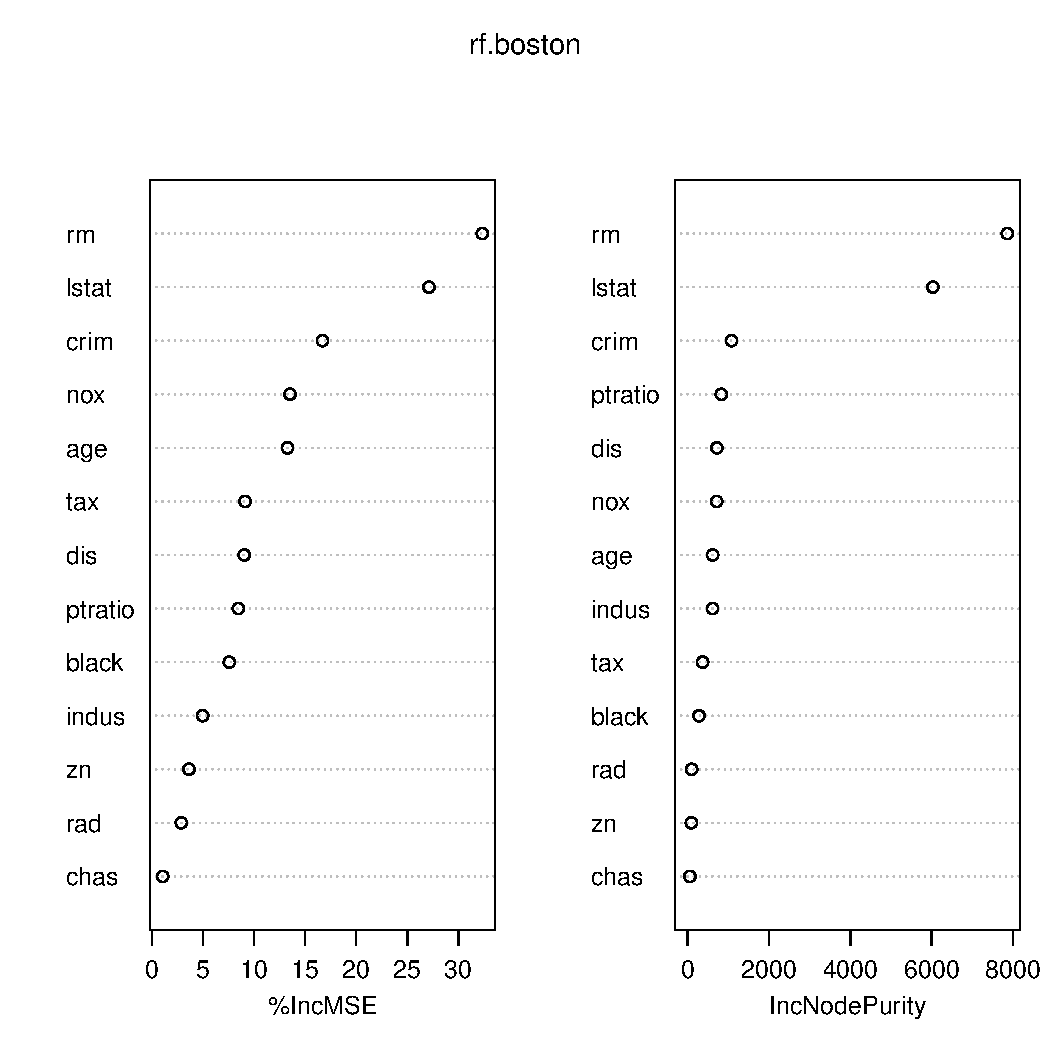
\includegraphics[width=\maxwidth]{figure/unnamed-chunk-23-1} 

\end{knitrout}

\newpage
\section{Boosting}

Here we use the \texttt{gbm} package, and within it \texttt{gbm()} function, to fit boosted regression trees to the \texttt{Boston} data set. We run \texttt{gbm()} with the option \texttt{distribution=``gaussian''} since this is a regression problem; if it were a binary classification problem, we would use \texttt{distribution=``bernoulli''}. The argument \texttt{n.trees=5000} indicates that we want 5000 trees, and the option \texttt{interaction.depth=4} limits the depth of each tree.

\begin{knitrout}
\definecolor{shadecolor}{rgb}{0.969, 0.969, 0.969}\color{fgcolor}\begin{kframe}
\begin{alltt}
\hlkwd{set.seed}\hlstd{(}\hlnum{1}\hlstd{)}
\hlstd{boost.boston}\hlkwb{=}\hlkwd{gbm}\hlstd{(medv}\hlopt{~}\hlstd{.,} \hlkwc{data}\hlstd{=Boston[train,],}
                 \hlkwc{distribution}\hlstd{=}\hlstr{"gaussian"}\hlstd{,} \hlkwc{n.trees}\hlstd{=}\hlnum{5000}\hlstd{,}
                 \hlkwc{interaction.depth}\hlstd{=}\hlnum{4}\hlstd{)}
\end{alltt}
\end{kframe}
\end{knitrout}

The \texttt{summary()} function produces a relative influence plot and also outputs the relative influence statistics.

\begin{knitrout}
\definecolor{shadecolor}{rgb}{0.969, 0.969, 0.969}\color{fgcolor}\begin{kframe}
\begin{alltt}
\hlkwd{summary}\hlstd{(boost.boston)}
\end{alltt}
\end{kframe}
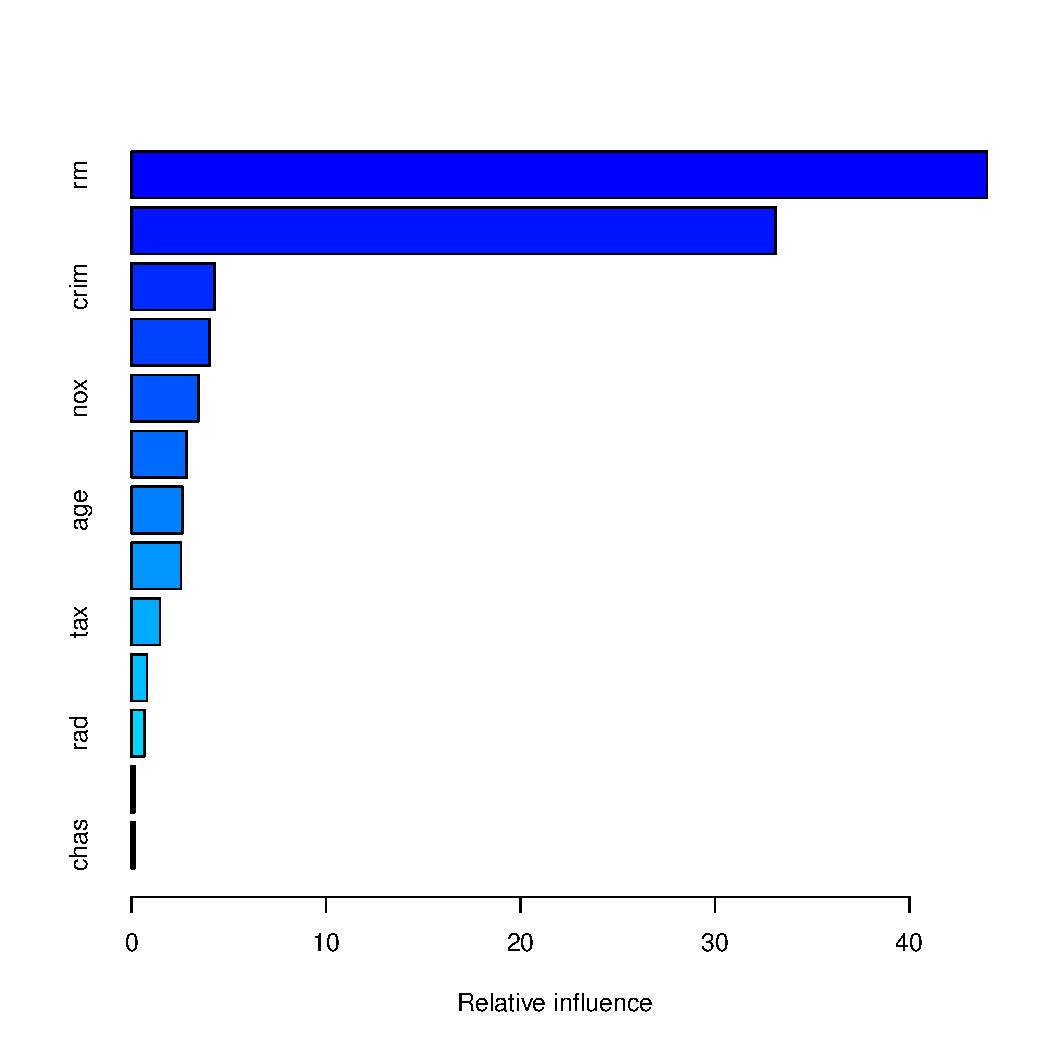
\includegraphics[width=\maxwidth]{figure/unnamed-chunk-25-1} 
\begin{kframe}\begin{verbatim}
##             var    rel.inf
## rm           rm 43.9919329
## lstat     lstat 33.1216941
## crim       crim  4.2604167
## dis         dis  4.0111090
## nox         nox  3.4353017
## black     black  2.8267554
## age         age  2.6113938
## ptratio ptratio  2.5403035
## tax         tax  1.4565654
## indus     indus  0.8008740
## rad         rad  0.6546400
## zn           zn  0.1446149
## chas       chas  0.1443986
\end{verbatim}
\end{kframe}
\end{knitrout}

We see that \texttt{lstat} and \texttt{rm} are by far the most important variables. We can also produce \textit{partial dependence plots} for these two variables. These plots illustrate the marginal effect of the selected variables on the response after \textit{integrating} out the other variables. In this case, as we might expect, median house prices are increasing with \texttt{rm} and decreasing with \texttt{lstat}.

\begin{knitrout}
\definecolor{shadecolor}{rgb}{0.969, 0.969, 0.969}\color{fgcolor}\begin{kframe}
\begin{alltt}
\hlkwd{par}\hlstd{(}\hlkwc{mfrow}\hlstd{=}\hlkwd{c}\hlstd{(}\hlnum{1}\hlstd{,}\hlnum{2}\hlstd{))}
\hlkwd{plot}\hlstd{(boost.boston,} \hlkwc{i}\hlstd{=}\hlstr{"rm"}\hlstd{)}
\end{alltt}
\end{kframe}
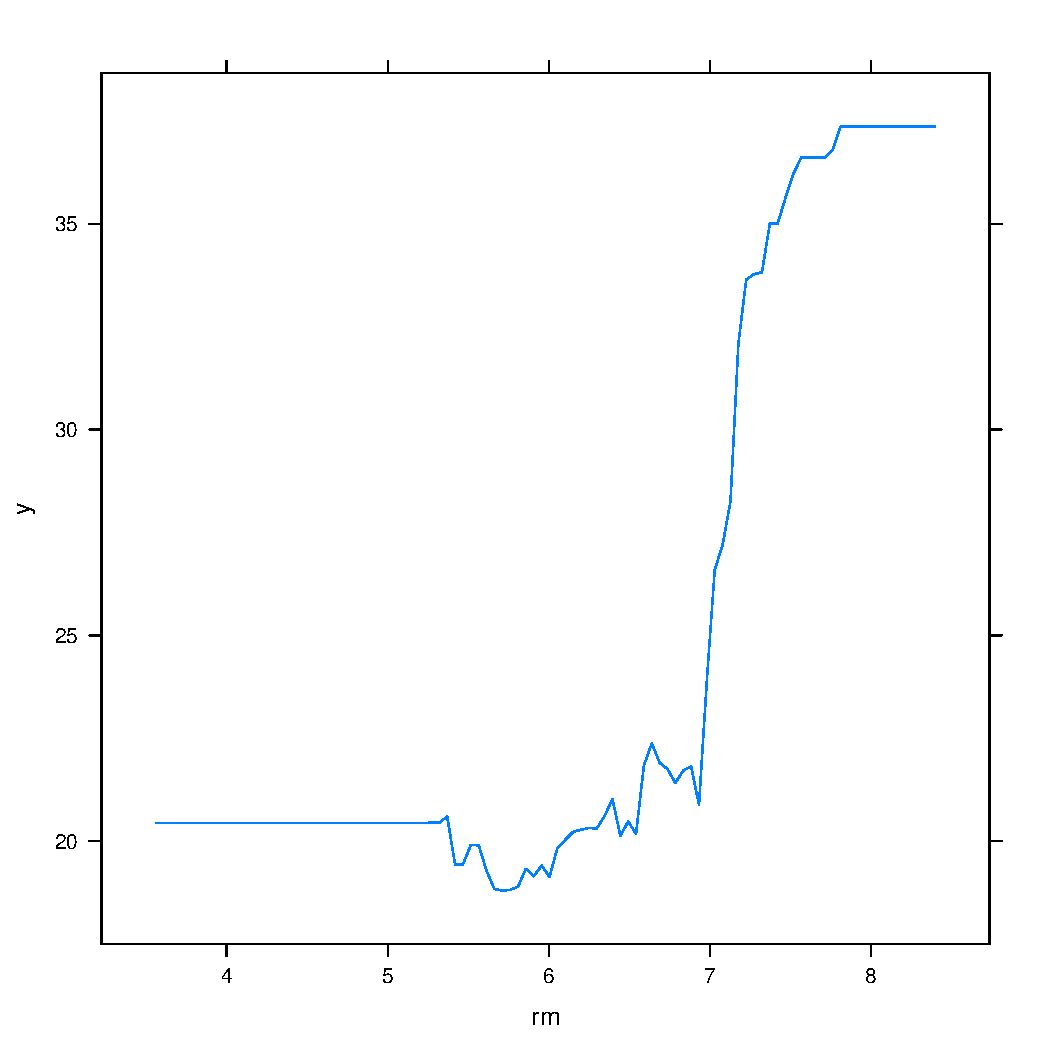
\includegraphics[width=\maxwidth]{figure/unnamed-chunk-26-1} 
\begin{kframe}\begin{alltt}
\hlkwd{plot}\hlstd{(boost.boston,} \hlkwc{i}\hlstd{=}\hlstr{"lstat"}\hlstd{)}
\end{alltt}
\end{kframe}
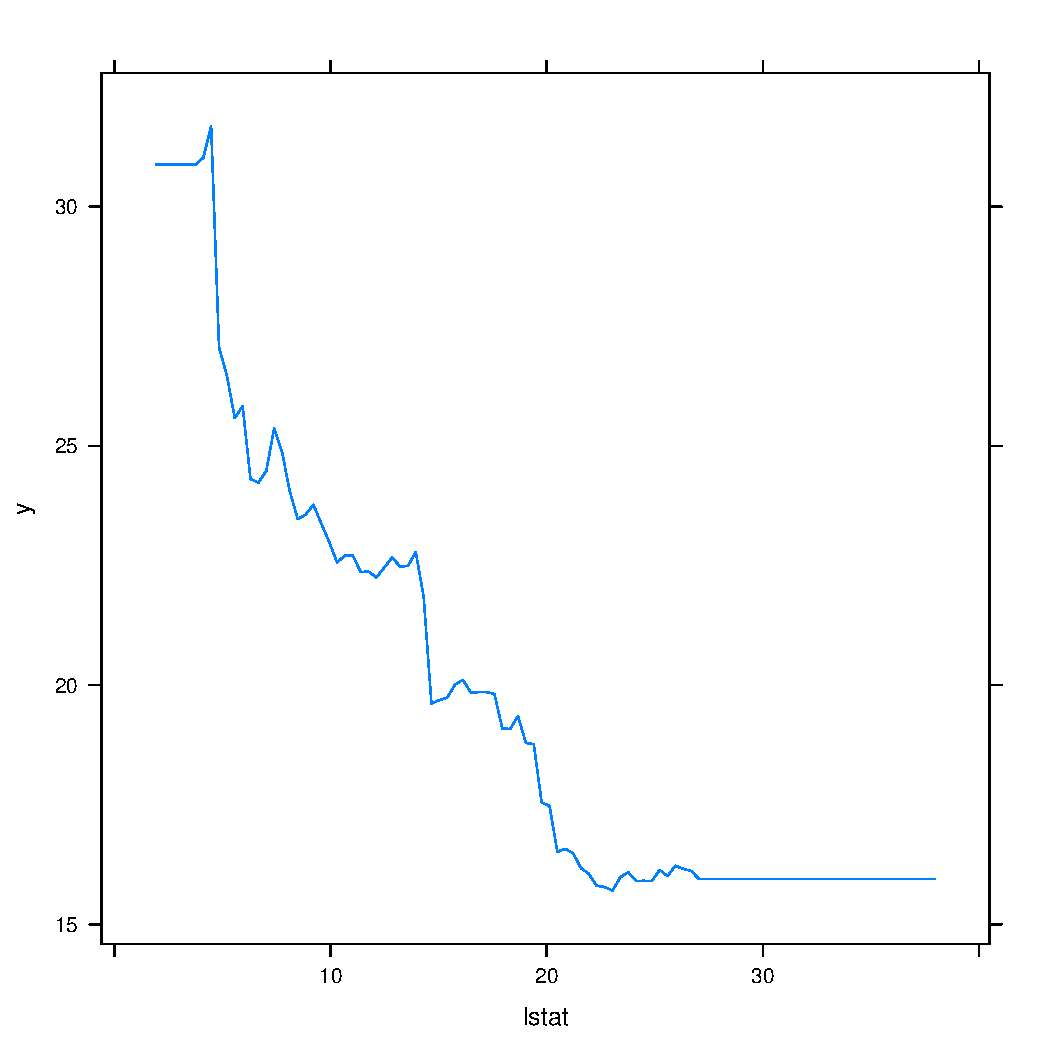
\includegraphics[width=\maxwidth]{figure/unnamed-chunk-26-2} 

\end{knitrout}

We now use the boosted model to predict \texttt{medv} on the test set:

\begin{knitrout}
\definecolor{shadecolor}{rgb}{0.969, 0.969, 0.969}\color{fgcolor}\begin{kframe}
\begin{alltt}
\hlstd{yhat.boost}\hlkwb{=}\hlkwd{predict}\hlstd{(boost.boston,} \hlkwc{newdata}\hlstd{=Boston[}\hlopt{-}\hlstd{train,],}
                   \hlkwc{n.trees}\hlstd{=}\hlnum{5000}\hlstd{)}
\hlkwd{mean}\hlstd{((yhat.boost}\hlopt{-}\hlstd{boston.test)}\hlopt{^}\hlnum{2}\hlstd{)}
\end{alltt}
\begin{verbatim}
## [1] 18.84709
\end{verbatim}
\end{kframe}
\end{knitrout}

The test MSE obtained is 11.8; similar to the test MSE for random forests and superior to that for bagging. If we want to, we can perform boosting with a different value of the shrinkage parameter $\lambda$. The default value is 0.0001, but this is easily modified. Here we take $\lambda = 0.2$.

\begin{knitrout}
\definecolor{shadecolor}{rgb}{0.969, 0.969, 0.969}\color{fgcolor}\begin{kframe}
\begin{alltt}
\hlstd{boost.boston} \hlkwb{=} \hlkwd{gbm}\hlstd{(medv}\hlopt{~}\hlstd{.,} \hlkwc{data} \hlstd{= Boston[train,],}
                   \hlkwc{distribution}\hlstd{=}\hlstr{"gaussian"}\hlstd{,}
                   \hlkwc{n.trees}\hlstd{=}\hlnum{5000}\hlstd{,}
                   \hlkwc{interaction.depth}\hlstd{=}\hlnum{4}\hlstd{,}
                   \hlkwc{shrinkage}\hlstd{=}\hlnum{0.2}\hlstd{,}
                   \hlkwc{verbose}\hlstd{=F)}
\hlstd{yhat.boost} \hlkwb{=} \hlkwd{predict}\hlstd{(boost.boston,}
                     \hlkwc{newdata}\hlstd{=Boston[}\hlopt{-}\hlstd{train,],}
                     \hlkwc{n.trees}\hlstd{=}\hlnum{5000}\hlstd{)}
\hlkwd{mean}\hlstd{((yhat.boost}\hlopt{-}\hlstd{boston.test)}\hlopt{^}\hlnum{2}\hlstd{)}
\end{alltt}
\begin{verbatim}
## [1] 18.33455
\end{verbatim}
\end{kframe}
\end{knitrout}

In this case, using $\lambda = 0.2$ leads to a slightly lower test MSE than $\lambda = 0.001$.
\end{document}
